\section{Дифференцируемые функции}

Всюду в этом разделе $I \subset \R$ -- невырожденный промежуток числовой прямой.

\begin{definition}
    Пусть $f: I \longrightarrow \R$, \ $a \in I$. \textit{Производной} функции $f$ в точке $a$ называется следующий предел:
    \[\lim_{x \rightarrow a} \frac{f(x) - f(a)}{x - a}\]
    Обозначается $f'(a)$, $\frac{df(a)}{dx}$.\\
    Если указанный предел конечен, то говорят, что функция $f$ \textit{дифференцируема} в точке $a$.
\end{definition}

Выражение $\frac{f(x) - f(a)}{x - a}$ называется \textit{разностным отношением}.

\begin{example}
    $f: \R \longrightarrow \R$, $f(x) = kx + b, \ \forall a \in \R$.
    \[f' = \lim_{x \rightarrow a} \frac{k(x - a)}{x - a} = k\]
\end{example}

\subsection{Геометрический смысл производной.}
Пусть функция $f$ дифференцируема в точке $a$. 

\[l_{\text{секущая}}: y = f(a) + \frac{f(t) - f(a)}{t - a} (x - a)\]
\[l_{\text{касательная}}: y = f(a) + f'(a)(x - a)\]
\[k_{\text{секущая}} = \frac{f(t) - f(a)}{t - a} \Rightarrow k_{\text{касательная}} = f'(a) \]

\begin{center}
    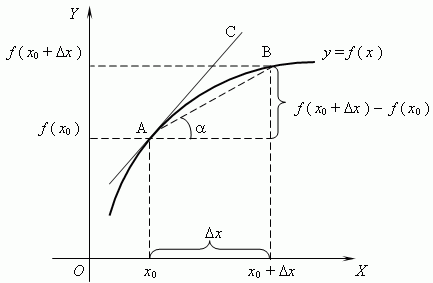
\includegraphics[width=0.55\textwidth]{print_1.png}
\end{center}

\begin{note}
    Угловой коэффициент секущей стремится к угловому коэффициенту касательной.
\end{note}

\begin{theorem}\hypertarget{th1}{О линейной аппроксимации}
    \\
    Пусть $f: I \longrightarrow \R$, \ $a \in I$.
    Функция $f$ дифференцируема в точке $a$ $\lra$ $\exists A \in \R$:
    \[f(x) = f(a) + A(x - a) + o(x - a), \ x \longrightarrow a,\]
\end{theorem}

\begin{proof}
    $\Rightarrow$ Пусть $f$ дифференцируема в $a$. Определим функцию $\alpha: I \rightarrow R$, $\alpha(x) = \frac{f(x) - f(a)}{x - a} - f'(a)$ при $ x \neq a$, и $\alpha(a)$ производная.
    Тогда $\lim_{x \to a} \alpha(x) = 0$ и $f(x) - f(a) = f'(a)(x - a) + \alpha(x)(x - a)$. Следовательно, выполнимо условие.
    \\
    $\Leftarrow$ Из условия следует, что $A + o(1) = \frac{f(x) - f(a)}{x - a}$. Переходя к пределу при $x \to a$, получаем $\exists \ f'(a) = A$, т.е. $f$ дифференцируема в точке $a$.
\end{proof}

\begin{corollary}
    Если $f$ дифференцируема в точке $a$, то $f$ непрерывна в $a$.
\end{corollary}

\begin{note}
    Обратное утверждение к следствию неверно.
    \\
    Функция $f: \R \to \R$, $f(x) = |x|$, непрерывна, но не дифференцируема в точке 0, так как
    \[\lim_{x \to \pm 0} \frac{f(x) - f(a)}{x - 0} = \lim_{x \to \pm 0} \frac{|x|}{x} = \pm 1.\]
\end{note}

Рассмотрение односторонних пределов приводит к следующему обобщению пределов.

\begin{definition}
    Пусть $f: I \to \R$, $a \in I$.
    \\
    $f_{+}'(a) = \lim_{x \to a + 0} \frac{f(x) - f(a)}{x - a}$ называется \textit{правой производной} $f$ в точке $a$.
    \\
    $f_{-}'(a) = \lim_{x \to a - 0} \frac{f(x) - f(a)}{x - a}$ называется \textit{левой производной} $f$ в точке $a$.
\end{definition}

\begin{note}
    Если $a$ -- внутренняя точка $I$, то $\exists \ f'(a) \lra f_{+}'(a) = f_{-}'(a)$. В этом случае все три предела равны.
    \\
    Если $a$ -- концевая точка $I$, то $f'(a)$ существует одновременно с соответствующей односторонней производной.
\end{note}

\begin{theorem}\hypertarget{th2}{}
    Пусть $f, g: I \to \R$, $a \in I$ и $\alpha, \beta \in \R$.
    Если $f$ и $g$ дифференцируемы в точке $a$, то в этой точке дифференцируемы $\alpha f + \beta g$, $f \cdot g$ и при условии $g \neq 0$ на $I$ также $\frac{f}{g}$. При этом 
    \begin{enumerate}
        \item $(\alpha f + \beta g)'(a) = \alpha f'(a) + \beta g'(a)$
        \item $(f \cdot g)'(a) = f'(a)g(a) + f(a)g'(a)$
        \item $(\frac{f}{g})(a) = \frac{f'(a)g(a) - f(a)g'(a)}{g^{2}(a)}$
    \end{enumerate}
\end{theorem}

\begin{proof}
    \begin{enumerate}
        \item Следует из свойств линейности предела.
        \item \[(f \cdot g)(x) - (f \cdot g)(a) = g(a)(f(x) - f(a)) + f(x)(g(x) - g(a))\]
    \[\lim_{x \to a} \frac{(f \cdot g)(x) - (f \cdot g)(a)}{x - a} = f'(a) g(a) + f(a) g'(a)\]
    -- непрерывна в точке $a$.
        \item Переходя к пределу при $x \to a$, получим
    \[\frac{(\frac{1}{g})(x) - (\frac{1}{g})(a)}{x - a} = \frac{1}{g(a) \cdot g(x)} \cdot \frac{g(a) - g(x)}{x - a},\]
    получим, что $g(x)$ дифференцируема в точке $a$.
    \end{enumerate}
\end{proof}

\begin{theorem}\hypertarget{th3}{Производная композиции}
    \\
    Пусть $I, J$ -- промежутки, $f: I \to J$, $g: J \to \R$. Если $f$ дифференцируема в точке $a \in I$ и $g$ дифференцируема в точке $b = f(a)$, то композиция $g_{o}f: I \to \R$ дифференцируема в точке $a$, причем
    \[(g_{o}f)'(a) = g'(b) \cdot f'(a)\]
\end{theorem}

\begin{proof}
    Определим функцию $h: J \to \R$, 
    \[ h(y) =
    \begin{cases}
        \frac{g(y) - g(b)}{y - b},       & \quad y \neq b\\
        g'(b),  & \quad y = b.
    \end{cases}
    \]
    Тогда $h$ непрерывна в точке $b$. Покажем, что $\forall x \in I$, $x \neq a$, выполнено
    \[\frac{(g_{o}f)(x) - (g_{o}f)(a)}{x - a} = h(f(x)) \cdot \frac{f(x) - f(a)}{x - a}\]
    Если $f(x) = f(a)$, то $0 = 0$. Если $f(x) \neq f(a)$, то равенство следует из того, что
    \[\frac{(g_{o}f)(x) - (g_{o}f)(a)}{x - a} = \frac{g(f(x)) - g(f(a)))}{f(x) - f(a)} \cdot \frac{f(x) - f(a)}{x - a}\]
    Перейдем к пределу
    \[\lim_{x \to a} \frac{(g_{o}f)(x) - (g_{o}f)(a)}{x - a} = g'(b)\cdot f'(a).\]
    (т.к. $h$ непрерывна в точке b, то по свойству предела композиции $\lim_{x \to a} h(f(x)) = h(b) = g'(b)$)
\end{proof}

\begin{theorem}\hypertarget{th4}{Производная обратной функции}
    \\
    Пусть $f: I \to \R$ непрерывна и монотонна на промежутке $I$. Если f дифференцируема в точке $a \in I$ и $f'(a) \neq 0$, то обратная функция $f^{-1}: f(I) \to I$ дифференцируема в точке $b = f(a)$, причем
    \[(f^{-1})'(b) = \frac{1}{f'(a)}\]
\end{theorem}

\begin{proof}
    По теореме об обратной функции на $J = f(I)$ определена функция $f^{-1}$, которая на $J$ непрерывна и строго монотонна. Следовательно, $f^{-1}(t) \to a$ при $t \to b$, $f^{-1}(t) \neq a$ при $t \neq b$
    \[\lim_{t \to b} \frac{f^{-1}(t) - f^{-1}(b)}{t - b} = \lim_{x \to a} \frac{f^{-1}(f(x))-f^{-1}(f(a))}{f(x) - f(a)} =\]
    \[ = \lim_{x \to a}\frac{x - a}{f(x) - f(a)} = \frac{1}{f'(a)}\]
\end{proof}

\newpage

\subsection{Таблица производных.}

\begin{enumerate}
    \item $c' = 0$
    \item $(a^{x})' = a^{x} \ln(a),$ при $a > 0, a \neq 1$
    \item $(\log_{a}x)' = \frac{1}{x \ln(a)},$ при $a > 0, a \neq 1$
    \item $(x^{\alpha})' = \alpha \cdot x^{\alpha - 1},$ при $\alpha \in \R$
    \item $(\sin{x})' = \cos{x}$
    \item $(\cos{x})' = - \sin{x}$
    \item $(\tg{x})' = \frac{1}{\cos^{2}{x}}$
    \item $(\ctg x)' = - \frac{1}{\sin^{2}{x}}$
    \item $(\arcsin{x})' = - (\arccos{x})' = \frac{1}{\sqrt{1 - x^{2}}},$ при $x \in (-1, 1)$
    \item $(\arctg {x})' = - (\arcctg{x})' = \frac{1}{1 + x^{2}}$
\end{enumerate}

\begin{proof}
    \begin{enumerate}
        \item По определению.
        \item По второму замечательному пределу $(e^{x})' = \lim_{t \to x} \frac{e^{t} - e^{x}}{t - x} = e^{x} \cdot \lim_{t \to x} \frac{e^{t - x} - 1}{t - x} = e^{x}.$\\
        $(a^{x})' = (e^{x \ln(a)})' = e^{x \ln(a)} \cdot (x \cdot \ln(a))' = a^{x} \ln(a).$
        \item $y = \log_{a}x \lra x = a^{y}$, по теореме о производной обратной функции получим: $(\log_{a}x)' = \frac{1}{(a^{y})'} = \frac{1}{a^{y} \ln(a)}.$
        \item $\alpha \in \Z \ \ (x^{n})' = n \cdot x^{n - 1}$ -- по определению. \\
        $\alpha \in \R \setminus \Z \ \ (x^{\alpha})' = (e^{\alpha \ln(x)})' = e^{\alpha \ln(x)} \frac{\alpha}{x} = \alpha \cdot x^{\alpha - 1}.$
        \item $(\sin x)' = \lim_{t \to x} \frac{\sin t - \sin x}{t - x} = \lim_{t \to x} \frac{\sin \frac{t - x}{2} \cos \frac{t + x}{2}}{\frac{t - x}{2}} = \cos x.$
        \item $(\cos x)' = (-1)\cdot \cos (\frac{\pi}{2} - x) = - \sin x.$
        \item $x \neq \frac{\pi}{2} + \pi k, \ k \in \Z$\\
        $(\tg x)' = (\frac{\sin x}{\cos x})' = \frac{\cos^{2}x + \sin^{2}x}{\cos^{2}x} = \frac{1}{\cos^{2}x}.$
        \item Аналогично пункту (7).
        \item $y = \arcsin x \lra x = \sin y \ \ y \in (-\frac{\pi}{2};\frac{\pi}{2})$\\
        $(\arcsin x)' = \frac{1}{(\sin y)'} = \frac{1}{\cos y} = \frac{1}{\sqrt{1 - \sin^{2}y}} = \frac{1}{\sqrt{1 - x^{2}}}.$
        \item Аналогично пункту (9).
    \end{enumerate}
\end{proof}

\begin{definition}
    Говорят, что функция $f$ дифференцируема на множестве $D$, если $f$ дифференцируема в каждой точке $D$. Функция $x \mapsto f'(x), \ \ x \in D$, называется \textit{производной} $f$ и обозначается $f'$. 
\end{definition}

\begin{corollary}
    Всякая элементарная функция дифференцируема во внутренних точках своей области определения, причем производная -- тоже элементарная функция.
\end{corollary}

\begin{definition}
    Пусть $\phi, \psi: T \to \R$, $\phi(T) = E$. Говорят, что функция $f: E \to \R$ параметрически задана системой
    \[
    \begin{cases}
        x = \phi (t),   & \quad t \in T\\
        y = \psi (t),  & \quad t \in T,
    \end{cases}
    \]
    если $\forall t_{1}, t_{2} \in T \ (\phi(t_{1}) = \phi(t_{2}) \Rightarrow \psi(t_{1}) = \psi(t_{2}))$ и $f(x) = \psi(t)$, где $x = \phi(t)$.
    Импликация верна, если функция $\phi$ обратима, при этом $f(x) = (\psi_{o}\phi^{-1})(x)$.
\end{definition}

\begin{corollary}
    Пусть $\phi$ непрерывна и строго монотонна на промежутке $T$. Если функции $\phi$ и $\psi$ дифференцируемы в точке $t$ и $\phi'(t) \neq 0$, то параметрически заданная функция $f = \psi_{o}\phi ^{-1}$ дифференцируема в точке $x = \phi(t)$, причем 
    \[f'(x) = \frac{\psi'(t)}{\phi'(t)}\]
\end{corollary}

\begin{proof}
    По правилам дифференцирования композиции и обратной функции имеем:
    \[f'(x) = (\psi_{o}\phi^{-1})'(x) = \psi'(\phi^{-1}(x))(\phi^{-1})'(x) =\]
    \[= \psi'(\phi^{-1}(x))\frac{1}{\phi'(\phi^{-1}(x))} = \frac{\psi'(t)}{\phi'(t)}\]
\end{proof}

